
\documentclass[10pt,a4paper]{article}
\usepackage[utf8]{inputenc}
\usepackage[italian]{babel}
\usepackage{amsmath}
\usepackage{amsfonts}
\usepackage{amssymb}
\usepackage{graphicx}
\usepackage{float}
\usepackage[left=2cm,right=2cm,top=2cm,bottom=2cm]{geometry}
\usepackage{booktabs}
\newcommand{\rem}[1]{[\emph{#1}]}
\newcommand{\exn}{\phantom{xxx}}
\newcommand{\abs}[1]{\lvert#1\rvert}
%\renewcommand{\thesubsection}{\thesection.\alph{subsection}}  %% use 1.a numbering
\usepackage{hyperref}
\usepackage{graphicx} 


\usepackage{setspace}

\title{\Huge \textbf{Esperienza Preliminare}}
\author{Johann Bandini, Sofia Manzini, Alessio Niccolai }
\date{01 Novembre 2026}

\begin{document}

\maketitle
\section{Abstract}
Si sono studiati i segnali in uscita di un sistema di tre fotomoltiplicaatori disposti in verticale uno sopra l'altro, utilizzando un discriminatore e due unità di coincidenza, al fine di stimare tramite il rapporto di coincidenze triple su doppie la quantità $P_{\text{pass}} \cdot \varepsilon$. 
\section{Introduzione}
Lo scopo dell'esperienza è la rivelazione di raggi cosmici mediante l'utilizzo di PMT (plastic scintillators coupled to photomultiplier tubes).
In particolare l'analisi si concentra sullo studio delle proprietà statistiche dei conteggi delle particelle rivelate, e sulla misurazione dell'efficienza di rivelazione di uno dei tre PMT.


In primo luogo, il PMT superiore è stato collegato all'oscilloscopio tramite cavo coassiale caratterizzato da un ritardo di 2\textit{ns}.\\
Successivamente, il PMT è stato alimentato con tensioni comprese tra gli 800V e i 1200V, incrementando la tensione di 100V ad ogni step. \\
Impostato il trigger dell'oscillosopio a -30,4\textit{mV}, è stato studiato l'andamento del rate di trigger in funzione della tensione di alimentazione del PMT, andando a registrare 6 misure per ogni valore di tensione.\\
Dopo aver effettuato le misure è stato scelto il punto di lavoro per il PMT a 1100V in quanto sul nostro rivelatore la frequenza aspettata di raggi cosmici è nell'ordine dei 50-100Hz. \singlespacing
La scelta è stata effettuata notando che le misure per voltaggi più alti restituivano dei valori della frequenza di scatti nell'ordine dei kHz, il ché era attribuibile quasi esclusivamente al noise-rate mentre le misure a voltaggi più bassi avevano una frequenza di scatti troppo bassa ($<$ 50Hz) che faceva presupporre la perdita della maggior parte dei raggi cosmici.
Inoltre il voltaggio è stato scelto comunque in modo da avere valori di frequenze di scatto maggiori di 100Hz in quanto successivamente, con l'utilizzo delle unità di coincidenza, la quasi totalità degli scatti accidentali sarà eliminata.

\section{Punto di lavoro}


\begin{table}[htbp]
    \centering
   
    \begin{tabular}{||c|c||}
        
       
    
     
        \hline   
        \textbf{Tensione nominale (V)} & \textbf{Media del rate di trigger (Hz)} \\
        \hline 
        900  & 18 ${\pm}$ 4 \\
        \hline
        1000 & 61 ${\pm}$ 6 \\
        \hline
        1050 & 160 ${\pm}$ 15 \\
        \hline
        1100 & 390 ${\pm}$ 35 \\
        \hline
        1200 & 2830 ${\pm}$ 50 \\
        \hline
    \end{tabular}
    \caption{Media di 6 misure del rate di trigger dell'oscilloscopio,
     in funzione della tensione di alimentazione del PMT.}
\end{table}


\begin{figure}[h!]
    \centering
    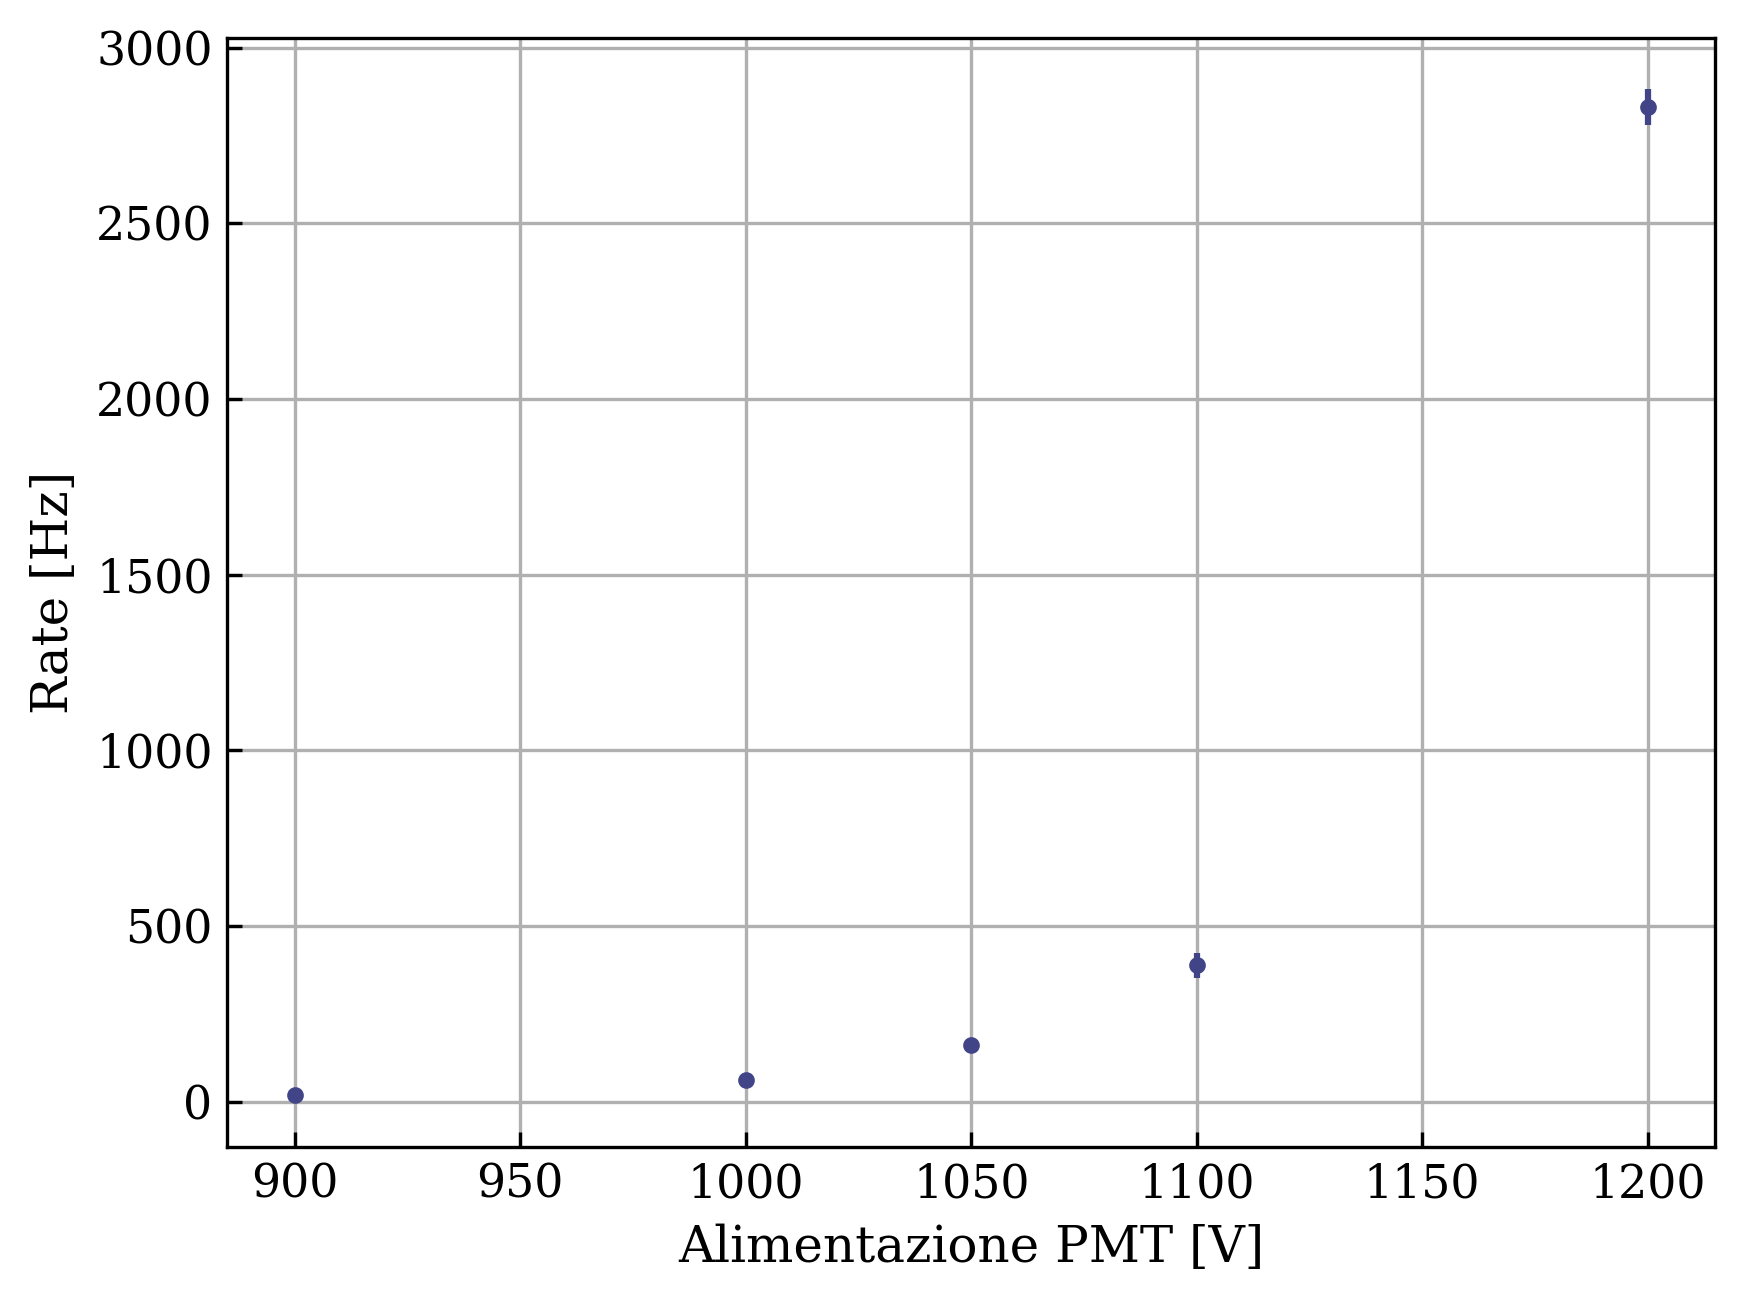
\includegraphics[width=0.7\textwidth]{rate_tensione.png}
    \caption{Rate di trigger in funzione della tensione di alimentazione del PMT.}
    \label{fig:rate_vs_v}
\end{figure}

Il rate di trigger in funzione della tensione di alimentazione del PMT è mostrato 
in figura \ref{fig:rate_vs_v}. \\ 
Si può notare che per tensioni più alte, il rate di trigger aumenta significativamente, indicando un aumento del rumore. 
D'altra parte, per tensioni più basse, il rate di trigger diminuisce,
suggerendo una perdita di eventi validi. Pertanto, la scelta del punto di 
lavoro a 1100V rappresenta un compromesso tra sensibilità e rumore.


\section{Discriminatore e conteggi in singola}
\subsection{Caratterizzazione del discriminatore}
Inserito il discriminatore nel crate NIM, il segnale in uscita dal PMT1 è stato connesso ad esso tramite cavo coassiale caratterizzato da un ritardo 3\textit{ns}. \\Il segnale in parallelo all'ingresso, e l'uscita del discriminatore, sono stati collegati rispettivamente ai canali 1 e 2 dell'oscilloscopio mediante cavi coassiali con ritardo di 2\textit{ns}.\\
Successivamente, il trigger del canale 1 è stato impostato a un valore di $-30\textit{mV}$ mentre la soglia del discriminatore ad un valore di -20\textit{mV}.
\singlespacing 
In questa configurazione il segnale del discriminatore sull'oscilloscopio presentava alcune anomalie:
a intervalli irregolari il livello logico 0 risultava traslato verso il basso rispetto a quello nominale; inoltre, nonostante la soglia del discriminatore fosse inferiore in modulo al valore di trigger, non vi era totale corrispondenza tra gli eventi triggerati dall'oscilloscopio e quelli rappresentati dal discriminatore.\\[6pt]
Tali anomalie erano da attribuirsi alle condizioni di funzionamento dell'alimentatore dei PMT, collegato direttamente al crate NIM, e operante in prossimità del limite massimo di corrente erogabile.
Con l'inserimento e l'attivazione del discriminatore, l'assorbimento complessivo superava saltuariamente la soglia di carico nominale del crate, generando instabilità e cadute di tensione sulle linee di alimentazione. \\Tali fluttuazioni privavano temporaneamente il discriminatore della corretta tensione di funzionamento, comportando le anomalie precedentemente descritte.\\[6pt]
La criticità è stata risolta successivamente con la sostituzione dell'alimentatore CAEN connesso al crate NIM con un alimentatore indipendente Wenzel N1130.\\[6pt]
Con l'apparato nuovamente in funzione è stata misurata la durata dell'impulso emesso dal discriminatore con i cursori dell'oscilloscopio. Il valore ottenuto è $(48 \pm 2)\textit{ns}$.
Inoltre è stato misurato il ritardo del segnale del discriminatore rispetto all'impulso del PMT1. La misura diretta tra i punti di inizio discesa dei due segnali ha fornito un valore di $(14 \pm 2)\textit{ns}$. \\Tuttavia, il discriminatore non scatta all'inizio della discesa del segnale, ma genera l'impulso in uscita soltanto quando la tensione d'ingresso scende al di sotto della soglia impostata di $-20\textit{mV}$. Valutando il ritardo a partire dall'istante in cui l'impulso del PMT1 raggiunge tale valore di soglia fino all'inizio del segnale di uscita, il ritardo effettivo del modulo si riduce a $(12 \pm 2)\textit{ns}$.
\\[6pt]L'incertezza di $\pm 2\textit{ns}$ è stata ottenuta raddoppiando l'errore associato al singolo cursore ($\pm 1\textit{ns}$), legato alla risoluzione del fondo scala utilizzato, così da considerare l'incertezza combinata su entrambi gli estremi dell'intervallo temporale.

\subsubsection{Effetto della soglia del discriminatore}
Nella tabella~\ref{tab:effetto_soglia} sono riportati i valori medi di frequenza misurati al variare della soglia del discriminatore, dove $s$ rappresenta la deviazione standard della media campionaria. All'aumentare del valore assoluto della soglia si osserva una progressiva riduzione del conteggio medio, dovuta all'esclusione dei segnali con ampiezza inferiore al livello impostato.
\begin{table}[h!]
  \centering

  \label{tab:effetto_soglia}
  \vspace{0.2cm}
  \begin{tabular}{||c|c||}
    \hline
    \textbf{Soglia [mV]} & \textbf{Rate di trigger [Hz]} \\
    \hline
    $-24 \pm 1$ & $410 \pm 50$ \\ \hline
    $-30 \pm 1$ & $300 \pm 30$ \\ \hline
    $-46 \pm 1$ & $118 \pm 15$ \\ \hline
    $-60 \pm 1$ & $46 \pm 16$ \\
    \hline
  \end{tabular}
    \caption{Frequenza di trigger media e sua deviazione standard della media campionaria in funzione della soglia del discriminatore.}
\end{table}

%In questa configurazione il segnale del discriminatore sull'oscilloscopio risultava incoerente con il segnale del PMT1: infatti, nonostante la soglia inferiore in modulo, non vi era totale corrispondenza tra gli eventi triggerati dall'oscilloscopio e quelli rappresentati dal discriminatore. Inoltre, sull'oscilloscopio il segnale del discriminatore presentava un livello di linea di base continuo e traslato verso il basso rispetto a quello nominale     



%Descrizione di come abbiamo collegato i PMT ai discriminatori e allo scaler, 
%e come abbiamo effettuato le misure di conteggio in singola.
%L'output dei tre PMT sono stati collegati ai discriminatori con cavi da 2ns, e allo scaler con cvi da 4ns
%Scelta soglia discriminatore, misura di ritaardo introdotto dal discriminatore,
%misura della larghezza del segnale in uscita dal discriminatore.

\subsection{Conteggi in singola}

I tre PMT sono stati connessi ai rispettivi canali del discriminatore tramite cavi coassiali da 2\textit{ns}, e successivamente i segnali discriminati sono stati inviati allo scaler attraverso cavi coassiali da 4\textit{ns}.\\
Impostata la soglia del discriminatore a -30\textit{mV}, sono stati registrati i conteggi in 10 secondi per ciascun PMT, ripetendo la misura 10 volte per ogni rivelatore.\\

Nella tabella \ref{tab:conteggi_singola} sono riportati i valori dei conteggi registrati per ciascun PMT, mentre in figura \ref{fig:conteggi_singola} sono rappresentati i valori medi dei conteggi con le relative incertezze, calcolate come deviazione standard della media campionaria.\\[6pt]


\begin{table}[htbp]
    \centering
    
    
    \begin{tabular}{|c|c|c|c|c|c|c|c|c|c|c|}
        \hline
       
         & \multicolumn{10}{c|} {\textbf{Conteggi in 10s}} \\
        \cline{2-11} 
        
        
        \hline
        \textbf{PMT1} & 3001 & 2670 & 2698 & 2777 & 2785 & 2913 & 2851 & 2963 & 2929 & 2769 \\
        \hline
        \textbf{PMT2} & 1158 & 1111 & 1141 & 1102 & 1121 & 1184 & 1136 & 1131 & 1132 & 1118 \\
        \hline
        \textbf{PMT3} & 2020 & 1975 & 1983 & 1902 & 1931 & 1996 & 2004 & 1963 & 1963 & 1985 \\
        \hline
    \end{tabular}
    \label{tab:conteggi_singola}
    \caption{Conteggi in singola misura con scaler.}
    \label{tab:conteggi_singola}
\end{table}



\begin{figure}[h!]
    \centering
    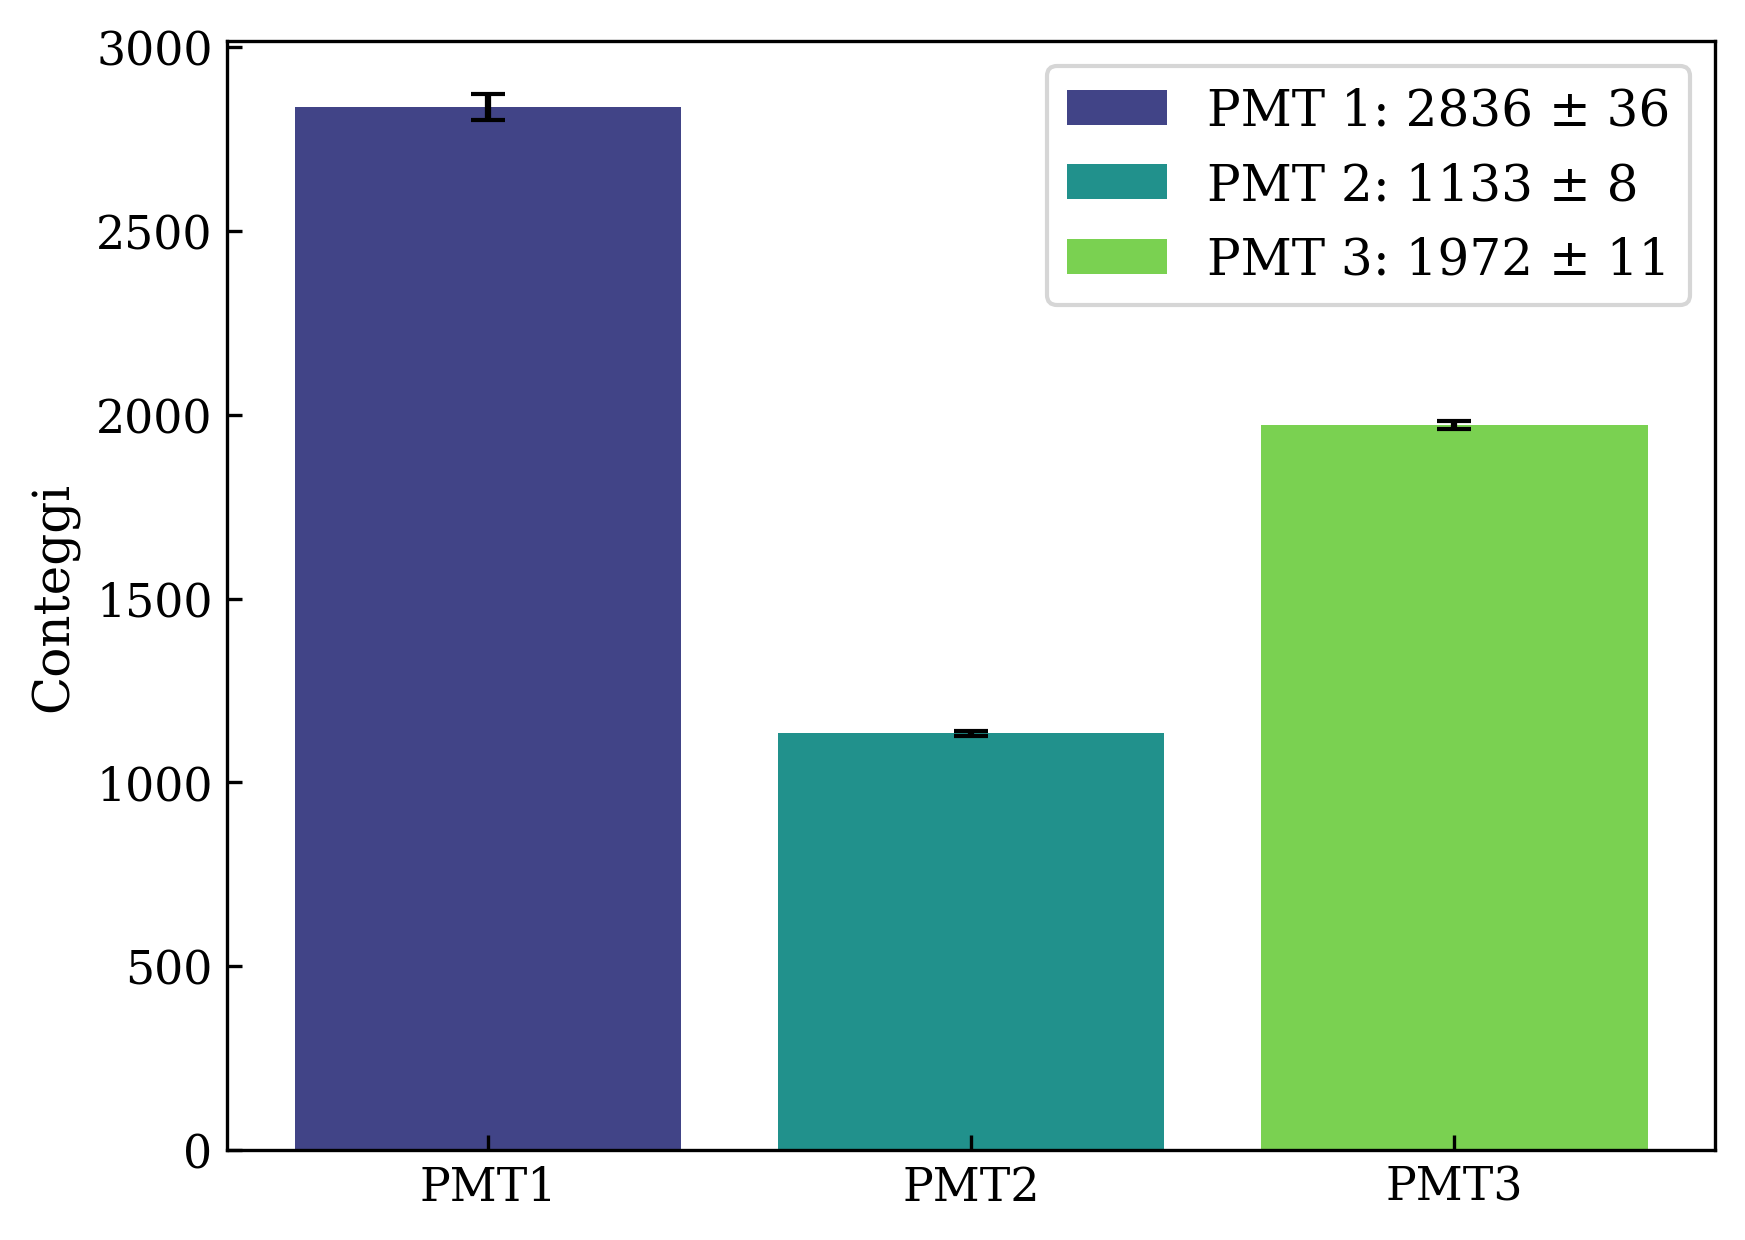
\includegraphics[width=0.8\textwidth]{conteggi in singola.png}
    \caption{Media dei conteggi 10 secondi per ogni PMT.}
    \label{fig:conteggi_singola}
\end{figure}


\clearpage

\section{Coincidenze}
I segnali discriminati dei tre PMT sono stati mandati in ingresso all'unità di coincidenza attraverso dei cavi da 2\textit{ns}, e la sua uscita è stata mandata al contatore con un altro cavo da 2\textit{ns}.\\
Sono stati attivati a 2 a 2 i canali dell'unità di coincidenza in modo da ottenere delle misure di coincidenze doppie per ciascuna delle combinazioni dei 3 PMT. Successivamente sono stati attivati tutti i canali per ottenere le misure delle coincidenze triple.

Questi sono i risultati ottenuti:


\begin{table}[htbp]
    \centering
    
    \begin{tabular}{|c|c|c|c|c|c|c|c|c|c|c|}
        \hline

         
       
         \textbf{Combinazione} & \multicolumn{10}{c|} {\textbf{Conteggi in 10s}} \\
        \cline{2-11} 
        
        
        \hline
        \textbf{1-2} & 43 & 36 & 36 & 40 & 47 & 33 & 39 & 45 & 35 & 44 \\
        \hline
        \textbf{1-3} & 18 & 23 & 20 & 9 & 13 & 18 & 23 & 19 & 28 & 17 \\
        \hline
        \textbf{2-3} & 67 & 63 & 59 & 70 & 54 & 80 & 66 & 52 & 59 & 80 \\
        \hline
        \textbf{1-2-3} & 14 & 8 & 15 & 14 & 18 & 10 & 15 & 28 & 13 & 27 \\
        \hline
    \end{tabular}
    \caption{Conteggi di coincidenze doppie e triple con unità di coincidenza.}
    \label{tab:coincidenze}
\end{table}

Si nota che, come aspettato, la combinazione che ha il rate minore di coincidenze doppie è proprio la 1-3 che ha i rivelatori più distanti,  inoltre la combinazione 1-2 ha un rate minore rispetto alla combinazione 2-3 perché nel nostro setup i rivelatori 1-2 sono più distanti fra loro rispetto ai rivelatori 2-3.\\
Le coincidenze triple, come aspettato, hanno rate minore rispetto a tutte le combinazioni delle coincidenze doppie.
\singlespacing

In figura \ref{fig:coincidenze} sono riportati i valori medi dei conteggi per ogni combinazione di coincidenze, con incertezze date dalla deviazione standard della media campionaria.


\begin{figure}[h!]
    \centering
    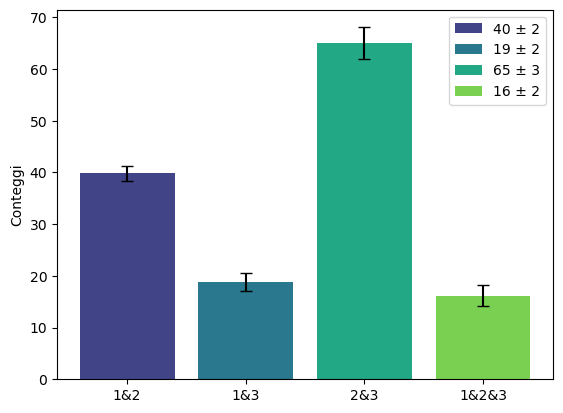
\includegraphics[width=0.75\textwidth]{coincidenze.png}
    \caption{Conteggi nelle coincidenze.}
    \label{fig:coincidenze}
\end{figure}


\newpage



\section{Stima dell'efficienza con coincidenze triple e doppie}
Per ottenere una stima dell'efficienza dello scintillatore centrale, si è valutato il rapporto fra gli eventi di coincidenza tripla e coincidenza doppia attraverso i rivelatori 1 e 3 acquisiti nella stessa unità di tempo, trascurando le coincidenze doppie accidentali (vedi appendice 1 e 2).\\[6pt]
Per fare ciò è stato necessario l'utilizzo di un altra unità di coincidenza che è stata inserita nel crate (opportunamente spegnendo l'alimentazione durante l'inserimento).\\[6pt]
Nella seconda unità di coincidenza sono state mandate in ingresso le uscite dei 3 discriminatori per effettuare il conteggio delle coincidenze triple mentre nella prima unità sono stati attivati solo i canali dei PMT 1 e 3 per effettuare il conteggio delle coincidenze doppie e le uscite sono state collegate allo scaler.\\[6pt]
Per fare in modo da non avere sfasamenti dei segnali introdotti dalla lunghezza dei cavi, le uscite dei 3 PMT sono state collegate al discriminatore con cavi da 3ns, le uscite del discriminatore alle unità di coincidenza con cavi da 2\textit{ns} e le uscite delle unità di coincidenza allo scaler con cavi da 4\textit{ns}.\\[6pt]
Utilizzando il punto di lavoro stabilito nella sezione 2 (alimentando quindi i 3 PMT a 1100V) è stata effettuata un acquisizione dalla durata di 1000s (è stato scelto un tempo lungo per aumentare il numero di acquisizioni e migliorare così l'errore sul rapporto triple doppie) e questi sono i risultati ottenuti:


\begin{table}[h!]
    \centering
    \begin{tabular}{||c|c|c||}
        \hline
        \textbf{Triple}  & \textbf{Doppie} & \textbf{Rapporto} \\
        \hline
        1697 & 2112 & 80.4 $\pm$ 0.9 \% \\
        \hline
        
    \end{tabular}
\label{tab:efficienza}

\end{table}

L’incertezza sul rapporto è data dalla distribuzione binomiale delle coincidenze triple sul numero di doppie fissate (vedi appendice 3).


\begin{figure}[h!]
    \centering
    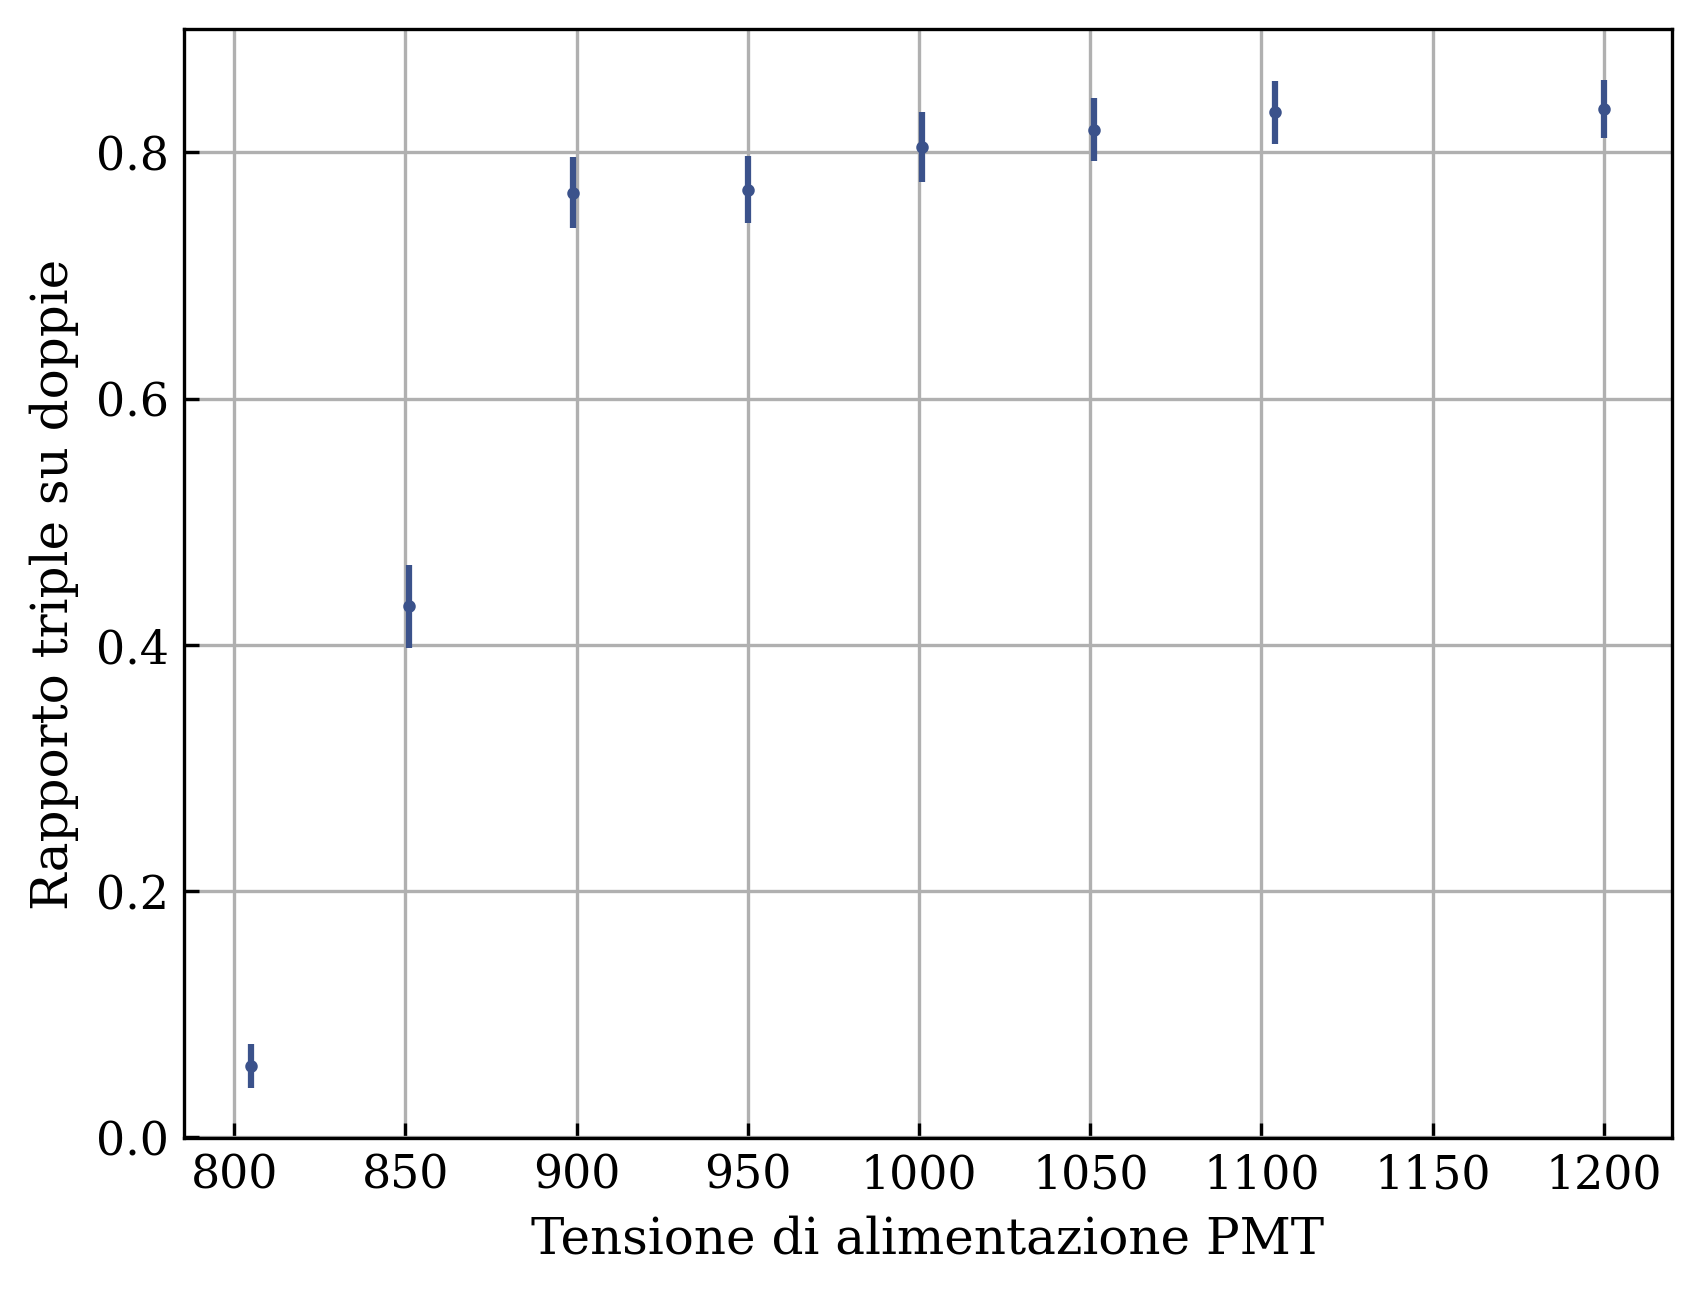
\includegraphics[width=0.75\textwidth]{efficienza_v.png}
    \caption{Andamento del rapporto triple su doppie al variare della tensione di alimentazione dei PMT.}
    \label{fig:efficienza_v}
\end{figure}

\subsection{Efficienza in funzione del punto di lavoro del PMT}

Le acquisizioni di triple e doppie sono state ripetute per diversi valori di alimentazione del PMT centrale.

Questi sono i risultati ottenuti:

\begin{table}[h!]
    \centering
    \begin{tabular}{||c|c|c||}
        \hline
        \textbf{Alimentazione PMT 2}  & \textbf{Triple} & \textbf{Doppie} \\
        \hline
        800V & 173 & 10  \\
        \hline
        850V & 218 & 94  \\
        \hline
        900V & 215 & 165  \\
        \hline
        950V & 239 & 184  \\
        \hline
        1000V & 194 & 156  \\
        \hline
        1050V & 226 & 185  \\
        \hline
        1100V & 209 & 174  \\
        \hline
        1150V & 252 & 210  \\
        \hline
        1200V & 243 & 203  \\
        \hline
        
    \end{tabular}
\label{tab:efficienza}

\end{table}



\section{Distribuzione conteggi}
Abbiamo registrato il numero di coincidenze triple in un periodo di 1 secondo, ripetendo la misura 55 volte per ricostriuire la distribuzione dei conteggi.
\singlespacing
In figura \ref{fig:fit poisson}, è riportato l'istrogramma della frequenza dei conteggi, e la poissoniana con media restituita dal fit dei minimi quadrati sui dati.
\\ Il rapporto della media aritmetica sulla varianza dei dati è $\text{media}/\text{varianza}=1.016 \approx 1$, come ci si aspetterebbe da una poissoniana.
\begin{figure}[h!]
    \centering
    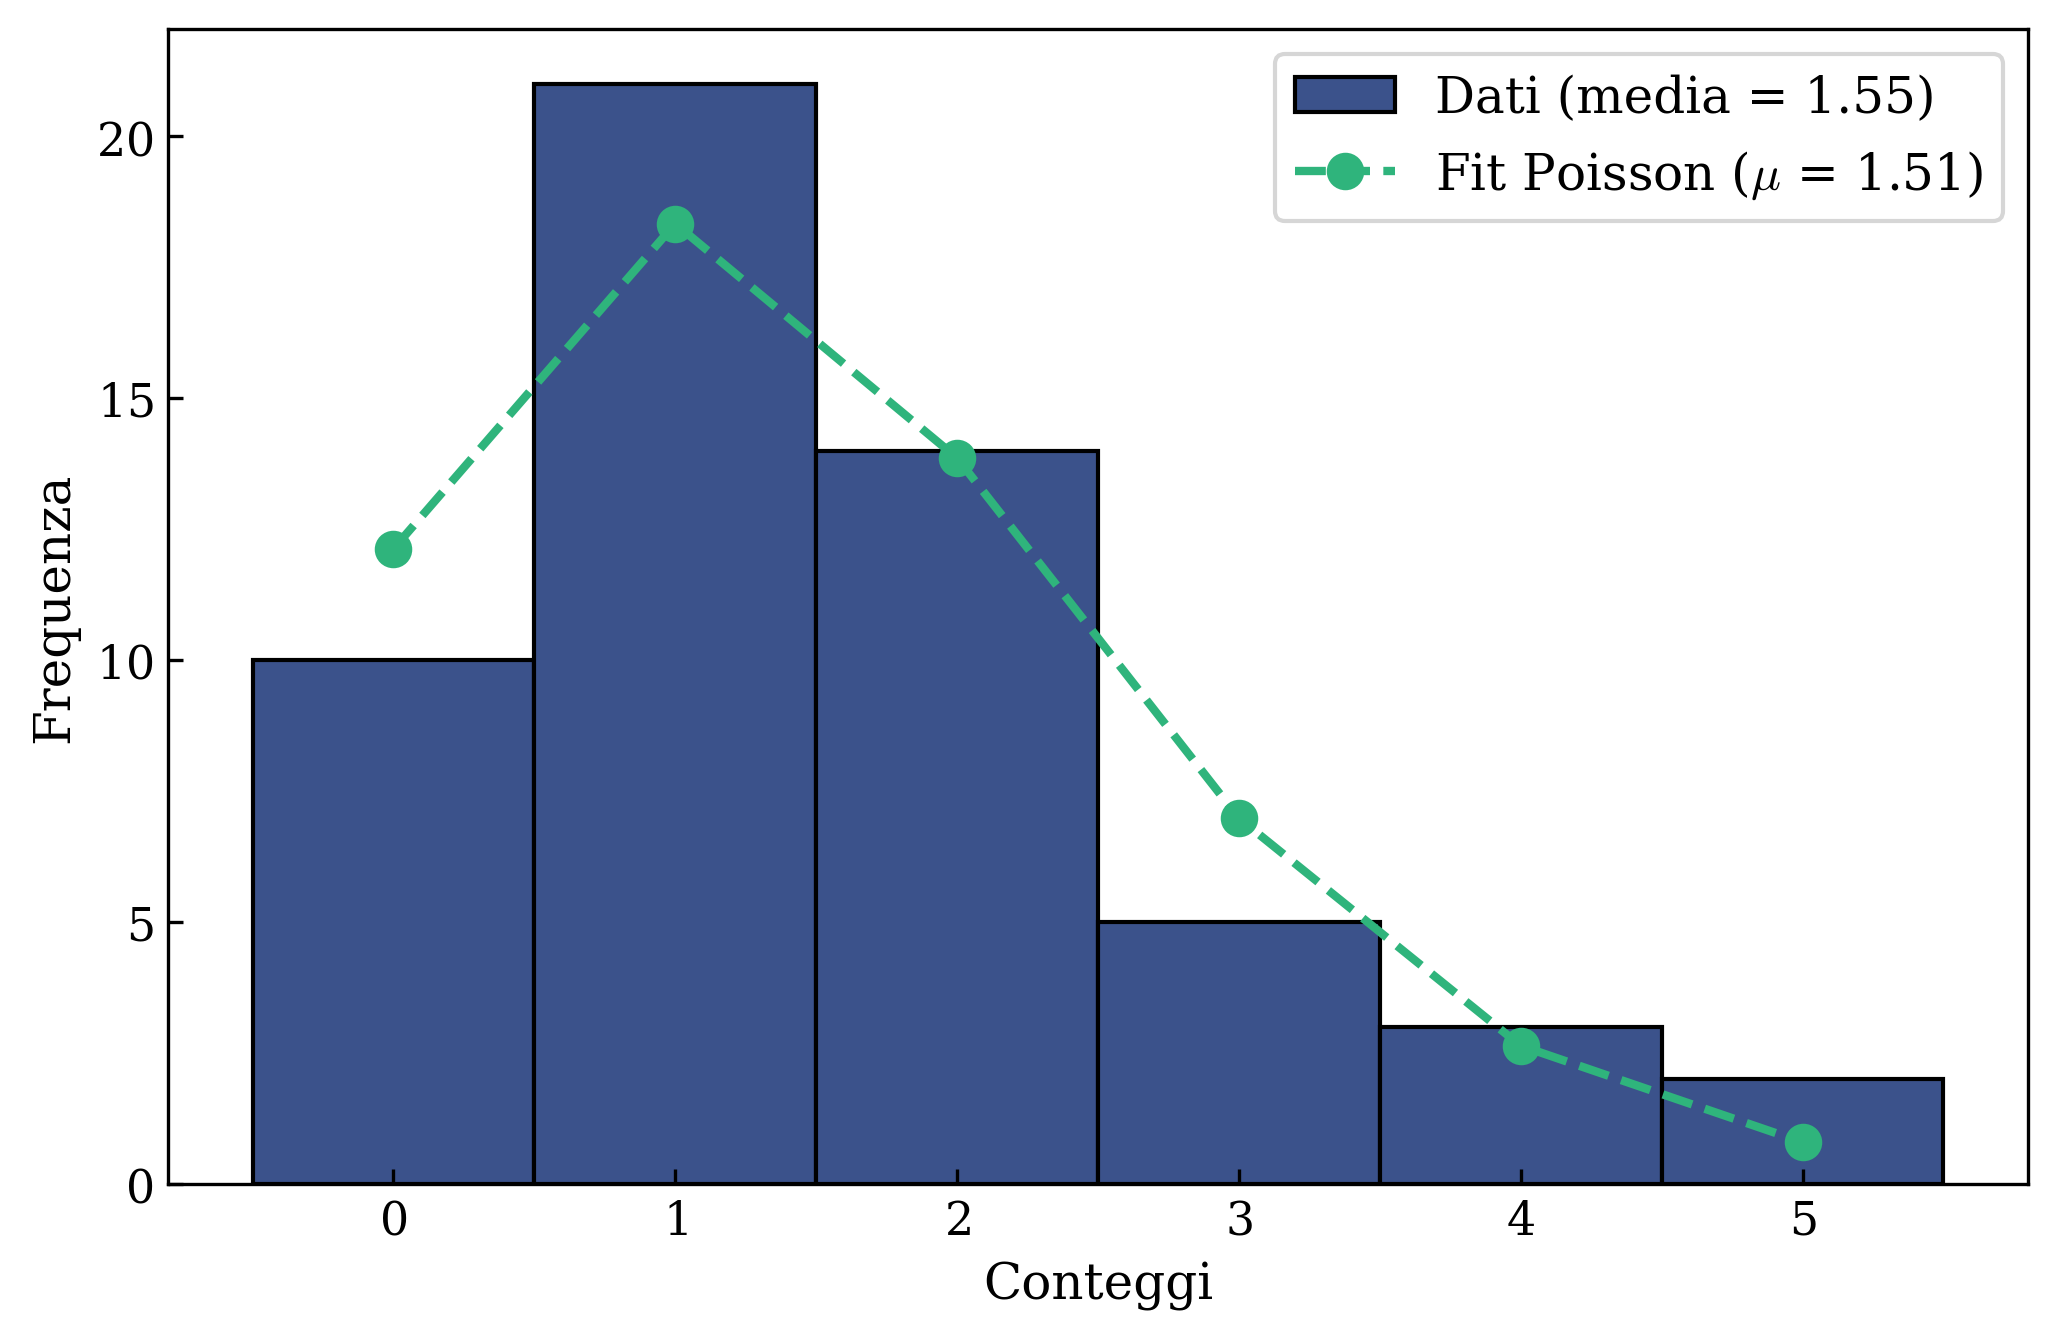
\includegraphics[width=0.75\textwidth]{fit poisson.png}
    \caption{Distribuzione conteggi coincidenze triple}
    \label{fig:fit poisson}
\end{figure}



\newpage


\section{Appendice}

\subsection{Rapporto triple/doppie e misure di efficienza}

Il rapporto tra coincidenze triple e doppie è legato all'efficienza dalla relazione:
$$\frac{\#\text{triple}}{\#\text{doppie}} = \frac{\#\text{doppie} \cdot P_{\text{pass}} \cdot \varepsilon}{\#\text{doppie}} = P_{\text{pass}} \cdot \varepsilon$$

Dove $\varepsilon$ è l'efficienza del rivelatore e $ P_{\text{pass}}$ è la probabilità che un raggio cosmico sia passato dal rivelatore condizionata dallo scatto della coincidenza doppia sugli altri due rivelatori.

Il rapporto triple su doppie si avvicina all'efficenza quanto più  $ P_{\text{pass}}$ è vicina ad 1 e questo dipende dalle caratteristiche geometriche dei 3 rivelatori.

La scelta di effettuare la misura sul rivelatore centrale deriva dal fatto che $P_{\text{pass}}$ è massimizzata in questa configurazione e il rapporto triple su doppie si avvicina il più possibile all'efficienza del rivelatore.

\subsection{Coincidenze doppie accidentali}

Il rate delle coincidenze doppie accidentali è dato dalla relazione:

$$R_a = R_1 \cdot R_3(\Delta t_1 + \Delta t_3 - 2\Delta t_s)$$

Dove $R_1$ e $R_3$ sono i rate in singola dei rivelatori 1 e 3, $\Delta t_1$ e $\Delta t_3$ sono le lunghezze temporali degli impulsi dei segnali discriminati dei rivelatori 1 e 3 e $\Delta t_s$ è il tempo di sovrapposizione minimo richiesto dall’unità di coincidenza.

Nel nostro caso $R_1 \approx 284 Hz$, $R_2 \approx 197 Hz$, $\Delta t_1 \approx \Delta t_3 \approx 48ns$ e $\Delta t_s \approx 2ns$ quindi ci aspettiamo un rate delle accidentali $R_a \approx 5.1\cdot 10^{-3} Hz$.
In un tempo $\Delta T = 100 s$ ci aspettiamo circa $\#accidentali = R_a \cdot \Delta T \approx 0.51$  mentre su $\Delta T = 1000 s$ ci aspettiamo $\#accidentali = R_a \cdot \Delta T \approx 5.1$ che sono trascurabili nella misura effettuata per il rapporto triple su doppie dove il numero di doppie misurato in 1000s è di 2112.

\subsection{Errore rapporto triple su doppie}

L'errore del rapporto triple su doppie è stato ottenuto considerando l'errore su una distribuzione binomiale con numero di doppie fissato.
Definendo:
$$\frac{\#\text{triple}}{\#\text{doppie}}  = P_{\text{pass}} \cdot \varepsilon = {\varepsilon}^{,} $$

L'errore su ${\varepsilon}^{,} $ è dato da:

$$\sigma_{{\varepsilon}^{,}} = \sqrt {\frac{{\varepsilon}^{,} \cdot (1- {\varepsilon}^{,})}{\#doppie} }$$

Nel nostro caso $\#doppie = 2112$ e $\varepsilon^{,} = 0.804$, quindi si ottiene $\sigma_{{\varepsilon}^{,}} = 9 \cdot 10^{-3}$.
\end{document}